\section{Pré-requis}
    \paragraph{JDK (Java Development Kit)}
    Pour un système d'exploitation Windows, l'utilisation de
    l'interpréteur LIR nécessite le jdk-15 ou une version ultérieure.

    \subsection{Installer le jdk-15}
    Sur la plateforme en ligne \verb|https://openjdk.java.net/projects/jdk/|,
    dans la rubrique "Release", télécharger la dernière version disponible du
    jdk.
    \\ Ranger le fichier .ZIP dans votre arborescence. Extraire les fichiers.

    \begin{center}
        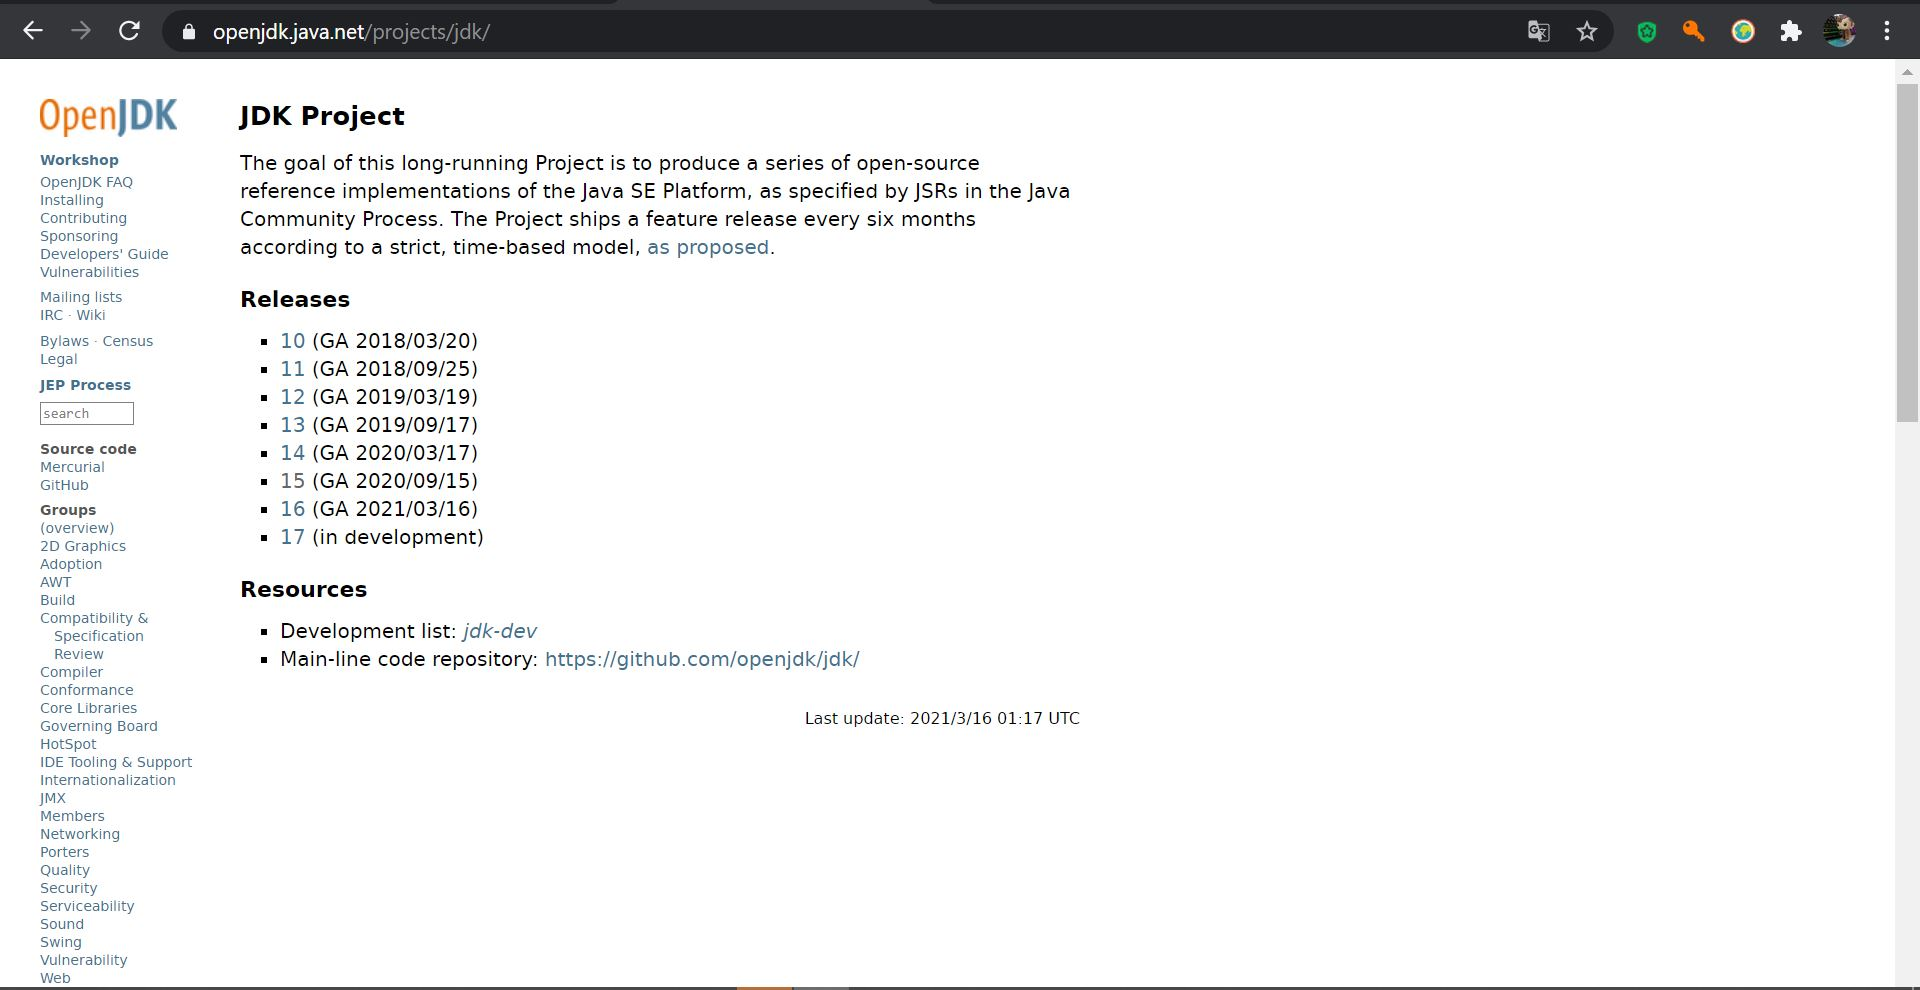
\includegraphics[width=\linewidth]{./img/installation-jdk.JPG}
    \end{center}

    \subsection{Configurer son environnement}
    \begin{enumerate}
        \item Ouvrir le Panneau de configuration Windows
        \item Accéder à la rubrique "Système et sécurité" puis "Système"
        \item Ouvrir la fenêtre "Paramètres système avancés"
        \item Ouvrir la fenêtre "Variable d'environnement"
        \item Sous la rubrique "Variables système", modifier la variable
              \verb|Path| en ajoutant ou modifiant le chemin d'accès au
              jdk-15 ou d'une version ultérieure.
    \end{enumerate}

    \begin{center}
        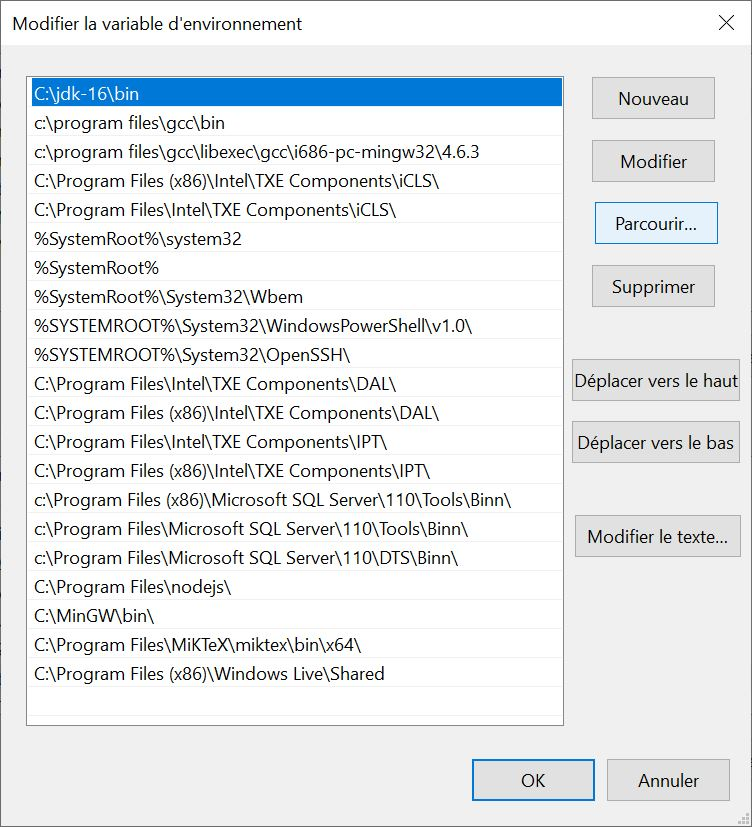
\includegraphics[height=8cm]{./img/installation-variable-environnement.JPG}
    \end{center}

    Pour vérifier de la prise en compte de la variable :
    \begin{enumerate}
        \item Ouvrir un invite de commande
        \item Entrer la commande \verb|javac| suivi de l'option \verb|-version|
    \end{enumerate}


    Exemple :
    \\ \verb|C:\user> javac -version|
    \\ \verb|javac version 15|

\section{Installation de l'Interpréteur LIR}
    Pour installer l'interpréteur LIR, suivre la démarche suivante :
    \begin{enumerate}
        \item Télécharger et ranger le fichier \verb|interpreteurLIR.zip |
              dans son arborescence
        \item Extraire le répertoire \verb|interpreteurLIR| du fichier .ZIP
    \end{enumerate}

    Pour lancer l'interpréteur LIR, il y a plusieurs possibilités :
    \begin{enumerate}
        \item Lancement à partir de l'explorateur de fichiers
        \item Lancement à partir d'un invite de commande
    \end{enumerate}

    \subsection{Lancement à partir de l'explorateur de fichiers}
    Possible si le chemin d'accès (path) au jdk-15 ou une version
    ultérieure est une variable système (cf. Configurer son environnement).
    Dans le répertoire \verb|interpreteurLIR|, sélectionner et ouvrir le fichier
    \verb|lanceInterpreteurLIR.bat|.

    \subsection{Lancement à partir d'un invite de commande}

    Si le chemin d'accès (path) au jdk-15 ou une version ultérieure est
    une variable système n'est pas une variable système, suivre l'étape 2.
    après l'ouverture de l'invite de commande.

    \begin{enumerate}
        \item Ouvrir un invite de commande
        \item \textit{optionnel } Définir une variable d'environnement à l'aide
              de la commande \verb|set path=| suivi du chemin d'accès au répertoire
              \verb|bin| de votre version du jdk.
              \\ Exemple : \verb|C:\user> set path=C:\jdk-15\bin|
        \item À l'aide de la commande \verb|cd| se placer dans le répertoire
              \verb|interpreteurLIR|
        \item Écrire \verb|lanceInterpreteurLIR.bat| ou alors
              \verb|java -jar interpreteurLIR.jar| pour lancer l'interpréteur
    \end{enumerate}

    Exemples 1 de lancement :
    \\ \verb|C:\user> javac -version|
    \\ \verb|javac version 8|
    \\ \verb|C:\user> set path=C:\jdk-15\bin|
    \\ \verb|C:\user>cd C:\user\Documents\chemin_d_acces\interpreteurLIR|
    \\ \verb|C:\user\Documents\chemin_d_acces\interpreteurLIR> lanceInterpreteurLIR.bat| \\
    \\ Exemple 2 de lancement :
    \\ \verb|C:\user> javac -version|
    \\ \verb|javac version 15|
    \\ \verb|C:\user>cd C:\user\Documents\chemin_d_acces\interpreteurLIR|
    \\ \verb|C:\user\Documents\chemin_d_acces\interpreteurLIR> java -jar interpreteurLIR.jar|






